\begin{figure}
\begin{center}
    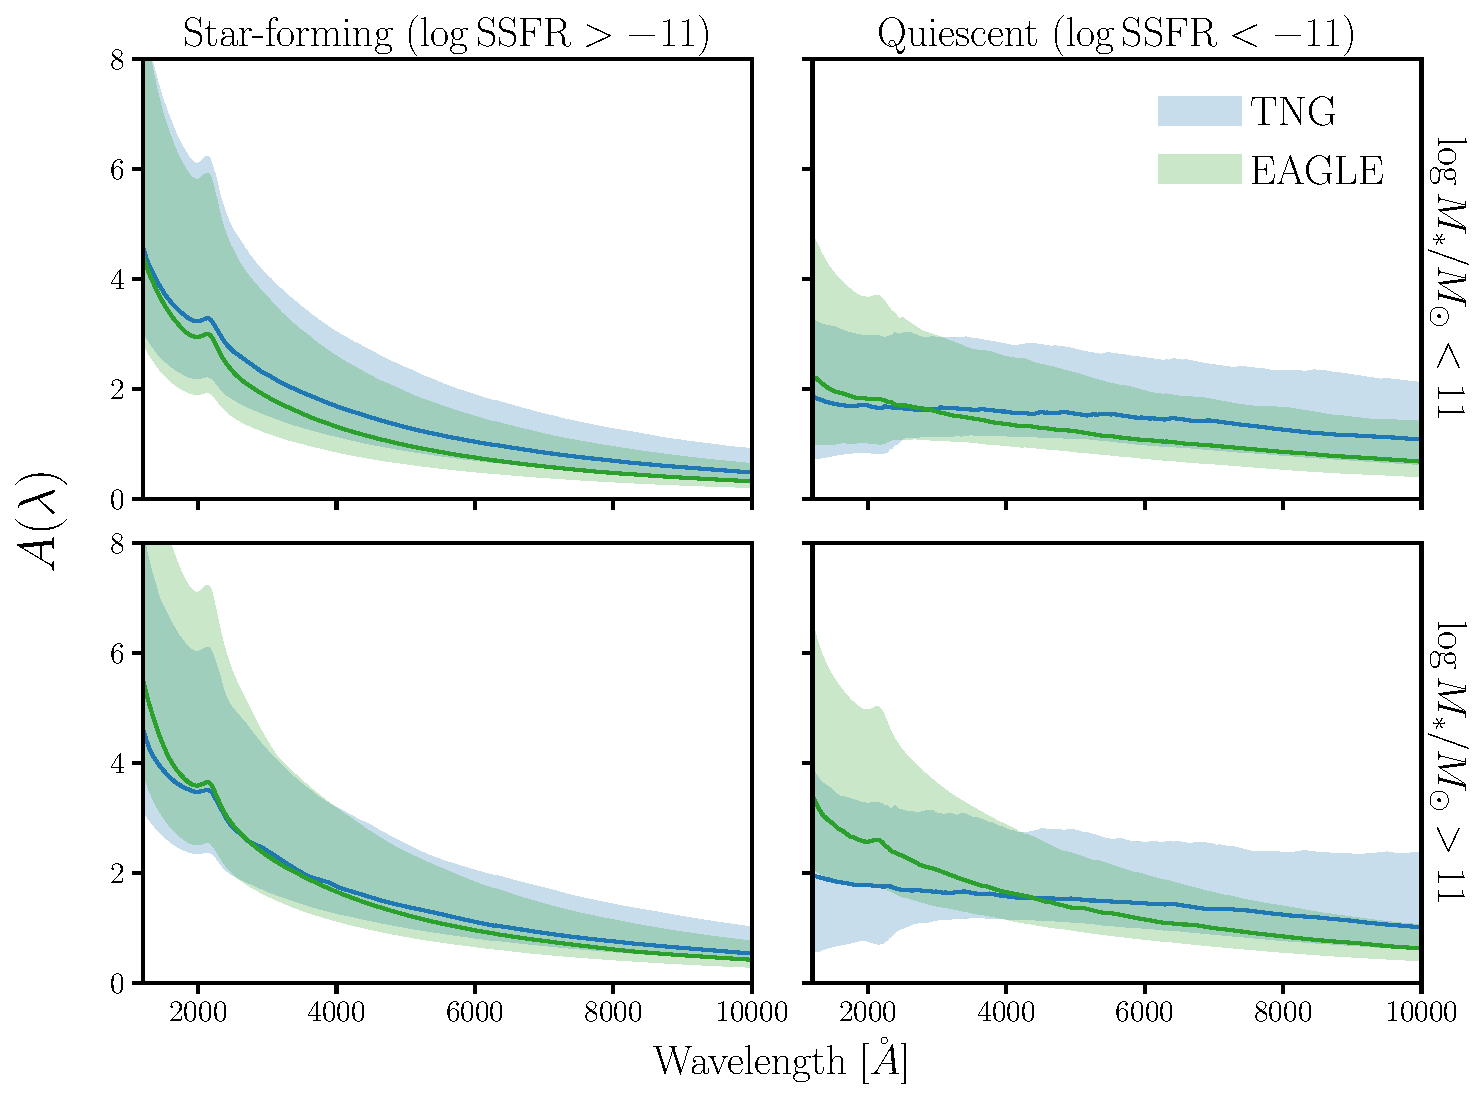
\includegraphics[width=0.85\textwidth]{figs/abc_attenuation_unormalized.pdf}
    \caption{\label{fig:raw_atten}
    Same as Figure~\ref{fig:atten} except the attenuation curves are not
    normalized at 3000$A$. Based on the \eda, quiescent galaxies have
    significant UV and optical dust attenuation. However, they have 
    significantly lower attenuation in the UV compared to star-forming 
    galaxies and have shallow attenuation curves overall.
    }
\end{center}
\end{figure}
\subsection{The Attenuation Curves of Quiescent Galaxies}  
We have demonstrated so far that the \eda~is able reproduce the observed UV and
optical color-magnitude relations and also predict dust attenuation curves
of star-forming galaxies consistent with observations and radiative transfer 
simulations. In addition, the \eda~also predicts dust attenuation curves of
quiescent galaxies. This is particularly valuable since there are many challenges 
to measuring attenuation curves for quiescent galaxies directly from observations. 
Methods that rely on IR luminosities can be contaminated by MIR emission from AGN
heating nearby dust~\citep{kirkpatrick2015}. Even SED fitting methods require 
accounting for AGN MIR emission~\citep{salim2016, leja2018, salim2018}. They
also struggle to tightly constrain dust attenuation for quiescent 
galaxies since they are limited by the degeneracies with star formation history and 
metallicity.

With a forward modeling approach, we circumvent these challenges. We derive the 
attenuation curves necessary for quiescent galaxy population in simulations to
reproduce the observed optical and UV photometry.  In right panels of
Figure~\ref{fig:atten}, we present the attenuation curves of quiescent galaxies 
predicted by the \eda~model for the median posterior parameter values of TNG (blue) 
and EAGLE (green). In the top and bottom panels, we present galaxies with 
$M_* < 10^{11} M_\odot$ and $M_* > 10^{11} M_\odot$, respectively. 
We define galaxies with $\log {\rm SSFR} < -11$ as quiescent. The right panels 
of Figure~\ref{fig:raw_atten} are the same as in Figure~\ref{fig:atten}, except
the attenuation curves are not normalized. 

For both TNG and EAGLE posteriors, the \eda~predicts significant dust attenuation 
in quiescent galaxies. Compared to star-forming galaxies, however, they have 
lower attenuation in the UV and much shallower attenuation curves. The amplitude 
of the attenuation is driven by the fact that both TNG and EAGLE --- without dust --- predict quiescent galaxies that are too 
luminous compared to observations. Hence, significant attenuation is necessary 
to lower their luminosity. Meanwhile, the shallow slope is driven by the
simulations predicting quiescent galaxies that are bluer in the optical but
redder in the UV than observations. The \eda~optically reddens the quiescent
galaxies but maintains a shallow enough slope to reproduce the UV
color-magnitude relation. This is also why TNG has a shallower slope than
EAGLE: TNG has an optically redder quiescent population and more quiescent
galaxies with high $\fnuv$ color. 

Given the challenges in observationally measuring attenuation curves of quiescent
galaxies, the predictions of the bestfit \eda~models for TNG and EAGLE again 
highlight the advantages of a forward modeling approach and provide valuable 
insights into dust attenuation in quiescent galaxies. \emph{Quiescent galaxies
have significant UV and optical attenuation with shallow slopes.} 

